% ============================================================
% Chapter 23: Hilbert's Problem 22 — Uniformization of Analytic Relations
% ============================================================

\chapter{Uniformization of Analytic Relations}

\begin{solvedbox}
\textbf{Resolved (1907--1913).} Paul Koebe (1907) and, independently, Henri Poincar\'e (1907) proved the uniformization theorem for simply connected Riemann surfaces. The general case follows as a corollary. Every analytic relation can be uniformized.
\end{solvedbox}

% -----------------------------------------------------------
\section{Historical Context}
% -----------------------------------------------------------

\subsection{Riemann's Vision}

In the mid-nineteenth century, Bernhard Riemann introduced a significant idea: to study complex-analytic functions not on flat subsets of the complex plane, but on \emph{curved surfaces} on which a complex structure could be defined. These objects, later named \textbf{Riemann surfaces} in his honor, arose naturally as the natural domains of multivalued functions such as $w = \sqrt{z}$ or $w = \log z$.

Riemann's significant achievement was his \emph{mapping theorem}, which he announced in his 1851 doctoral dissertation:

\begin{theorem}[Riemann Mapping Theorem]
Let $\Omega \subset \mathbb{C}$ be a simply connected open set that is not all of $\mathbb{C}$. Then there exists a biholomorphic map (a conformal equivalence) $f \colon \Omega \to \mathbb{D}$, where $\mathbb{D} = \{z \in \mathbb{C} : |z| < 1\}$ is the open unit disk.
\end{theorem}

This theorem says that, from the viewpoint of complex analysis, every simply connected region in the plane (other than the plane itself) ``looks like'' the unit disk. The proof, which Riemann sketched using methods from physics, was made rigorous by Karl Weierstrass and later by Poincar\'e and others. But Riemann's vision went further. He asked: \emph{can every Riemann surface be described in some standard, uniform way?}

\subsection{The Concept of Uniformization}

The word ``uniformization'' has a precise meaning here. A Riemann surface $X$ is \emph{uniformized} if it can be represented as a quotient
\[
    X \;\cong\; \widetilde{X}\, /\, \Gamma,
\]
where $\widetilde{X}$ is a ``simple'' domain---one of the three simply connected Riemann surfaces we will meet shortly---and $\Gamma$ is a discrete group of automorphisms (bijective conformal self-maps) acting freely on $\widetilde{X}$.

The dream, then, is this: given any Riemann surface, however complicated, find a simply connected ``covering'' space and a group that ``folds'' it down to produce the original surface. If this can always be done, every Riemann surface has a uniform description.

% -----------------------------------------------------------
\section{The Problem}
% -----------------------------------------------------------

Hilbert stated his twenty-second problem as follows:

\begin{problem_statement}
Can every analytic relation (Riemann surface) be uniformized? Can it be represented as a quotient $\widetilde{X}/\Gamma$, where $\widetilde{X}$ is a standard simply connected Riemann surface and $\Gamma$ a discrete group of automorphisms?
\end{problem_statement}

To make this precise, we need a few definitions.

% -----------------------------------------------------------
\section{What Is a Riemann Surface?}
% -----------------------------------------------------------

\begin{definition}[Riemann surface]
A \textbf{Riemann surface} is a connected 1-dimensional complex manifold; equivalently, a connected Hausdorff space with an \emph{atlas}: for each $p$, a neighborhood $U\ni p$ and a homeomorphism $\varphi:U\to V\subset\mathbb{C}$, with holomorphic transition maps.
\end{definition}

In simpler terms, a Riemann surface is a surface that ``locally looks like'' a piece of the complex plane, and the different ``pieces'' fit together in a way that respects the complex structure.

Here are the key examples to keep in mind:

\begin{itemize}
    \item \textbf{The Riemann sphere $\widehat{\mathbb{C}}$.} Take the complex plane and add a point at infinity. Topologically this is the two-dimensional sphere $S^2$, and it has a natural complex structure making it into a Riemann surface. The Riemann sphere is the \emph{compactification} of $\mathbb{C}$: every bounded sequence has a limit point, and every meromorphic function on $\widehat{\mathbb{C}}$ is a rational function.

    \item \textbf{The complex plane $\mathbb{C}$.} A Riemann surface with the simplest possible structure: every point has a neighborhood biholomorphic to an open disk in $\mathbb{C}$.

    \item \textbf{The unit disk $\mathbb{D}$.} $\mathbb{D} = \{z \in \mathbb{C} : |z| < 1\}$. As a Riemann surface, $\mathbb{D}$ is biholomorphic to the upper half-plane $\mathbb{H} = \{\tau \in \mathbb{C} : \operatorname{Im}(\tau) > 0\}$ via the Cayley transform $z \mapsto \frac{z-i}{z+i}$.

    \item \textbf{Tori.} A torus $\mathbb{C}/\Lambda$, where $\Lambda$ is a lattice in $\mathbb{C}$, is a compact Riemann surface of genus~$1$. It arises by gluing opposite sides of a parallelogram. Every compact Riemann surface of genus~$1$ is biholomorphic to such a quotient.

    \item \textbf{Hyperbolic surfaces.} Compact surfaces of genus $g \geq 2$ carry a Riemann surface structure, but---as we will see---they cannot be realized as quotients of $\mathbb{C}$. They require the disk $\mathbb{D}$.
\end{itemize}

\begin{remark}
The \emph{genus} of a Riemann surface is the number of ``handles'' on the underlying topological surface. The sphere has genus~$0$, the torus genus~$1$, and so on. As we will see, the genus determines which of the three standard models appears in the uniformization.
\end{remark}

% -----------------------------------------------------------
\section{The Three Simply Connected Surfaces}
% -----------------------------------------------------------

The classification of simply connected Riemann surfaces is the heart of the uniformization theorem. There are exactly three possibilities, up to biholomorphic equivalence:

\begin{enumerate}
    \item \textbf{The Riemann sphere $\widehat{\mathbb{C}}$.}\; This is the \emph{elliptic} case. The sphere is compact, and its group of automorphisms is the \emph{M\"obius group}
    \[
        \operatorname{PSL}(2,\mathbb{C}) \;=\; \left\{ z \;\mapsto\; \frac{az + b}{cz + d} \;:\; a,b,c,d \in \mathbb{C},\; ad - bc = 1 \right\}.
    \]
    Any Riemann surface whose universal cover is the sphere is itself a quotient of the sphere by a finite group of M\"obius transformations acting without fixed points.

    \item \textbf{The complex plane $\mathbb{C}$.}\; This is the \emph{parabolic} case. The automorphism group of $\mathbb{C}$ consists of all affine maps $z \mapsto az + b$ with $a \neq 0$.

    \item \textbf{The unit disk $\mathbb{D}$ (equivalently, the upper half-plane $\mathbb{H}$).}\; This is the \emph{hyperbolic} case. The automorphism group of $\mathbb{D}$ is the group $\operatorname{PSL}(2,\mathbb{R})$ of real M\"obius transformations
    \[
        z \;\mapsto\; \frac{az + b}{cz + d}, \qquad a,b,c,d \in \mathbb{R},\; ad - bc = 1.
    \]
    This group acts by isometries of the \emph{Poincar\'e metric} $ds = \frac{2\,|dz|}{1 - |z|^2}$ on $\mathbb{D}$, which makes $\mathbb{D}$ into a model of \emph{hyperbolic geometry}.
\end{enumerate}

These three models---sphere, plane, and disk---are the ``building blocks'' from which all Riemann surfaces are assembled.

% -----------------------------------------------------------
\section{The Uniformization Theorem}
% -----------------------------------------------------------

The resolution of Hilbert's Problem~22 is the following important theorem, due independently to Koebe and Poincar\'e.

\begin{theorem}[Koebe--Poincar\'e Uniformization Theorem, 1907]
\label{thm:uniformization}
Every simply connected Riemann surface is biholomorphic to exactly one of the following three domains:
\[
    \widehat{\mathbb{C}}, \qquad \mathbb{C}, \qquad \text{or} \qquad \mathbb{D}.
\]
\end{theorem}

In other words, if $X$ is a simply connected Riemann surface, then $X$ is conformally equivalent to the sphere, the plane, or the disk---and no other possibilities exist. The three models are mutually inequivalent: the sphere is compact, the plane is parabolic (its Green's function is identically zero), and the disk is hyperbolic (it admits a bounded nonconstant holomorphic function).

\subsection{The General Uniformization Theorem}

Theorem~\ref{thm:uniformization} is for simply connected surfaces. The general case follows:

\begin{corollary}[General Uniformization Theorem]
\label{cor:general-uniformization}
Every Riemann surface $X$ is biholomorphic to a quotient
\[
    X \;\cong\; \widetilde{X}\, /\, \Gamma,
\]
where $\widetilde{X}$ is one of $\widehat{\mathbb{C}}$, $\mathbb{C}$, or $\mathbb{D}$, and $\Gamma$ is a discrete group of automorphisms of $\widetilde{X}$ acting freely (without fixed points) and properly discontinuously.
\end{corollary}

The idea is simple: take the universal cover $\widetilde{X} \to X$ of the Riemann surface. By the Uniformization Theorem for simply connected surfaces, $\widetilde{X}$ must be one of the three standard models. The fundamental group $\pi_1(X)$ then acts on $\widetilde{X}$ by deck transformations, and these deck transformations are automorphisms of $\widetilde{X}$.

\subsection{Which Surface Gets Which Model?}

For a compact Riemann surface of genus $g$, the uniformization is determined by the genus:

\begin{itemize}
    \item $g = 0$: the surface is the sphere $\widehat{\mathbb{C}}$ itself (elliptic).
    \item $g = 1$: the surface is a torus $\mathbb{C}/\Lambda$, a quotient of the plane (parabolic).
    \item $g \geq 2$: the surface is $\mathbb{D}/\Gamma$, a quotient of the disk (hyperbolic).
\end{itemize}

This trichotomy---sphere, plane, disk---corresponds to the three geometries of constant curvature: positive, zero, and negative.

% -----------------------------------------------------------
\section{Fuchsian Groups and Their Quotients}
% -----------------------------------------------------------

The most interesting case of uniformization---and the one with the richest geometry---is the hyperbolic case, where $\Gamma \subset \operatorname{PSL}(2,\mathbb{R})$.

\begin{definition}[Fuchsian group]
A \textbf{Fuchsian group} is a discrete subgroup $\Gamma \subset \operatorname{PSL}(2,\mathbb{R})$, the group of orientation-preserving isometries of the hyperbolic plane.
\end{definition}

Fuchsian groups are the discrete groups of automorphisms of the disk that appear in the uniformization of hyperbolic surfaces. They generalize the lattice translations that uniformize tori.

\subsection{Examples of Fuchsian Groups}

\paragraph{Example 1: Lattices (Parabolic Case).}
Before diving into the hyperbolic case, recall the simpler parabolic example. Let $\Lambda = \mathbb{Z} \oplus \mathbb{Z}\tau$ (with $\operatorname{Im}(\tau) > 0$) be a lattice in $\mathbb{C}$. The group $\Lambda$ acts on $\mathbb{C}$ by translations $z \mapsto z + \lambda$ for $\lambda \in \Lambda$. This action is free and properly discontinuous, and the quotient $\mathbb{C}/\Lambda$ is a torus. Here the ``Fuchsian group'' is the group of translations---abelian and easy to understand.

\paragraph{Example 2: The Modular Group $\operatorname{PSL}(2,\mathbb{Z})$.}
The group $\operatorname{PSL}(2,\mathbb{Z})$ of integer M\"obius transformations
\[
    z \;\mapsto\; \frac{az + b}{cz + d}, \qquad a,b,c,d \in \mathbb{Z},\; ad - bc = 1,
\]
is the prototypical Fuchsian group. It acts on the upper half-plane $\mathbb{H}$. The quotient $\mathbb{H}/\operatorname{PSL}(2,\mathbb{Z})$ is a non-compact Riemann surface---in fact, it is the moduli space of elliptic curves. It is not a compact surface, but rather a ``pillow'' with three orbifold points. This example is central to number theory and modular forms.

\paragraph{Example 3: Compact Quotients $\mathbb{H}/\Gamma$.}
For $g \geq 2$, there exist Fuchsian groups $\Gamma$ such that $\mathbb{H}/\Gamma$ is a compact Riemann surface of genus $g$. These groups are generated by $2g$ elements $\alpha_1, \beta_1, \ldots, \alpha_g, \beta_g$ satisfying the single relation
\[
    [\alpha_1, \beta_1] \cdots [\alpha_g, \beta_g] = 1,
\]
where $[\alpha, \beta] = \alpha \beta \alpha^{-1} \beta^{-1}$ is the commutator. Such groups can be realized as \emph{Schottky groups} or as fundamental domains in $\mathbb{H}$ with side-pairing transformations, following a construction due to Fricke and Klein.

\begin{figure}[htbp]
\centering
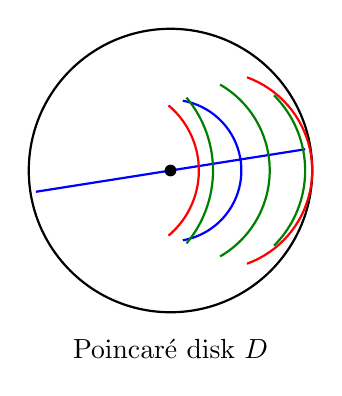
\begin{tikzpicture}[scale=1.8]
  \draw[thick] (0,0) circle (1);
  \draw[blue,thick] (0,0) -- (0.95,0.15);
  \draw[blue,thick] (-0.95,-0.15) -- (0,0);
  \draw[blue,thick,domain=-80:80,samples=40,variable=\t]
    plot ({0.5*cos(\t)},{0.5*sin(\t)});
  \draw[red,thick,domain=-70:70,samples=40,variable=\t]
    plot ({0.3+0.7*cos(\t)},{0.7*sin(\t)});
  \draw[red,thick,domain=-50:50,samples=40,variable=\t]
    plot ({-0.4+0.6*cos(\t)},{0.6*sin(\t)});
  \draw[green!50!black,thick,domain=-60:60,samples=40,variable=\t]
    plot ({0.7*cos(\t)},{0.7*sin(\t)});
  \draw[green!50!black,thick,domain=-40:40,samples=40,variable=\t]
    plot ({-0.5+0.8*cos(\t)},{0.8*sin(\t)});
  \draw[green!50!black,thick,domain=-45:45,samples=40,variable=\t]
    plot ({0.2+0.75*cos(\t)},{0.75*sin(\t)});
  \node at (0,0) [circle,fill,inner sep=1.5pt]{};
  \node[below] at (0,-1.12) {Poincar\'e disk $\mathbb{D}$};
\end{tikzpicture}
\caption{Poincar\'e disk model of hyperbolic geometry. Geodesics are circular arcs orthogonal to the boundary circle $\partial \mathbb{D}$. Blue arcs are diameters through the center; red and green arcs are circles orthogonal to the boundary.}
\label{fig:poincare-disk}
\end{figure}

\subsection{The Poincar\'e Disk Model}

The unit disk $\mathbb{D}$ with the metric
\[
    ds^2 \;=\; \frac{4\,|dz|^2}{(1 - |z|^2)^2}
\]
is a model of \emph{hyperbolic geometry}. In this model:

\begin{itemize}
    \item \textbf{Points} are points of $\mathbb{D}$.
    \item \textbf{Geodesics} (``hyperbolic lines'') are arcs of circles orthogonal to the unit circle, plus diameters of $\mathbb{D}$.
    \item \textbf{Distances} are measured by the hyperbolic metric, which blows up near the boundary $|z|=1$.
    \item \textbf{Angles} are the same as Euclidean angles (the metric is conformal).
\end{itemize}

The isometries of this metric are precisely the elements of $\operatorname{PSL}(2,\mathbb{R})$. These are the M\"obius transformations that map $\mathbb{D}$ to itself.

\begin{remark}
Hyperbolic geometry differs from Euclidean geometry in a fundamental way: the parallel postulate fails. Given a line $\ell$ and a point $p$ not on $\ell$, there are \emph{infinitely many} hyperbolic lines through $p$ that do not meet $\ell$---and indeed, they fall into three families (ultraparallel, asymptotic, and limiting parallel). This was Bolyai's and Lobachevsky's significant discovery.
\end{remark}

% -----------------------------------------------------------
\section{The Importance of Uniformization}
% -----------------------------------------------------------

The uniformization theorem is one of the key results of complex analysis and geometry, with significant connections across mathematics:

\begin{enumerate}
    \item \textbf{Classification of Riemann surfaces.} The theorem reduces the study of \emph{all} Riemann surfaces to three cases, each governed by a well-understood group of automorphisms. Complex analysis on a Riemann surface is transformed into the study of discrete group actions on standard domains.

    \item \textbf{Hyperbolic geometry.} The uniformization of surfaces of genus $g \geq 2$ provides concrete realizations of hyperbolic surfaces. Every such surface carries a unique hyperbolic metric in its conformal class (by the Gauss--Bonnet theorem, its total curvature is $-2\pi\chi = -2\pi(2 - 2g) < 0$). The Fuchsian group $\Gamma$ is the \emph{deck transformation group} of the hyperbolic universal cover.

    \item \textbf{Algebraic geometry.} Every compact Riemann surface is the same thing as a smooth projective algebraic curve over $\mathbb{C}$. Uniformization thus gives a significant connection between complex analysis, hyperbolic geometry, and algebraic geometry.

    \item \textbf{Number theory.} The modular group $\operatorname{PSL}(2,\mathbb{Z})$ and its subgroups are central to the theory of modular forms, elliptic curves, and the Langlands program. The quotient $\mathbb{H}/\operatorname{PSL}(2,\mathbb{Z})$ parametrizes isomorphism classes of elliptic curves, linking uniformization to arithmetic geometry.

    \item \textbf{Teichm\"uller theory.} The space of all complex structures on a surface of genus $g \geq 2$ is the \emph{Teichm\"uller space}, which can be understood as the space of Fuchsian representations of the fundamental group, modulo conjugation. This is a cornerstone of modern low-dimensional topology and geometric group theory.
\end{enumerate}

\begin{quote}
\textit{``The uniformization theorem is one of those rare results that, once understood, changes the way you see the entire subject. It says that the world of Riemann surfaces, however wild it may seem, is built from just three bricks---the sphere, the plane, and the disk---glued together by discrete groups.''}
\end{quote}

% -----------------------------------------------------------
\section{Summary}
% -----------------------------------------------------------

Hilbert asked whether every analytic relation (Riemann surface) can be uniformized---that is, represented as a quotient of a standard simply connected domain by a discrete group of automorphisms. The answer is yes. The Koebe--Poincar\'e uniformization theorem (1907) classifies simply connected Riemann surfaces into three types---$\widehat{\mathbb{C}}$, $\mathbb{C}$, and $\mathbb{D}$---and the general case follows by passing to the universal cover. The theorem unifies complex analysis, hyperbolic geometry, and algebraic geometry in a single, notable statement.

% -----------------------------------------------------------
\section*{Common Questions}
% -----------------------------------------------------------

\begin{description}[font=\bfseries, leftmargin=2em, style=nextline]

\item[Q: What does ``uniformization'' mean---why is that word used?]\hfill\\
``Uniformize'' means to make uniform or single. A multivalued function like $\sqrt{z}$ is not a genuine function in the usual sense (one input, one output). Uniformization finds a single domain (the universal cover) and a parametrization that turns the multivalued relation into an ordinary single-valued function---a ``uniform'' coordinate system for the whole surface.

\item[Q: Why are there exactly three simply connected Riemann surfaces?]\hfill\\
This is the Uniformization Theorem itself. By the Riemann mapping theorem, any simply connected region in $\mathbb{C}$ is either the disk or the plane (or the sphere if compact). The significant part is that the disk, the plane, and the sphere are mutually non-isomorphic: the sphere is compact, the plane admits no bounded nonconstant holomorphic function (Liouville), and the disk admits one (the identity). No fourth type exists.

\item[Q: How does uniformization connect to hyperbolic geometry?]\hfill\\
Every Riemann surface of genus $g \geq 2$ is uniformized by the disk, which carries a natural hyperbolic metric. The group $\Gamma$ that identifies sides of a fundamental domain consists of isometries of this metric. So these surfaces inherit a complete hyperbolic structure---they are ``hyperbolic surfaces.'' The Uniformization Theorem thus says that almost all Riemann surfaces are fundamentally geometric objects.

\item[Q: What does ``genus'' have to do with the choice of model?]\hfill\\
The Euler characteristic $\chi = 2 - 2g$ determines the sign of curvature. Sphere ($g=0$, $\chi=2$) has positive curvature and uniformizes itself. Torus ($g=1$, $\chi=0$) has zero curvature and uniformizes as $\mathbb{C}/\Lambda$. Higher genus ($g \geq 2$, $\chi < 0$) has negative curvature and uniformizes as $\mathbb{D}/\Gamma$. The genus tells you which of the three geometries the surface carries.

\item[Q: Is the uniformization theorem constructive?]\hfill\\
In principle, yes---Koebe and Poincar\'e gave existence proofs that produce the uniformizing map. In practice, for a specific Riemann surface (like a given algebraic curve $y^2 = x^3 + ax + b$), constructing the uniformization explicitly is extremely difficult and often involves special functions like the modular lambda function or theta functions.

\item[Q: What is a Fuchsian group?]\hfill\\
A Fuchsian group is a discrete subgroup of $\mathrm{PSL}(2,\mathbb{R})$, the group of orientation-preserving isometries of the hyperbolic plane. When you uniformize a genus $g \geq 2$ surface as $\mathbb{D}/\Gamma$, the group $\Gamma$ is Fuchsian. The group generates the surface by gluing edges of a fundamental polygon in the hyperbolic disk.

\end{description}

% -----------------------------------------------------------
\section{Exercises}
% -----------------------------------------------------------

\begin{enumerate}

    \item \textbf{The Cayley transform.} Verify that the map $w = \frac{z - i}{z + i}$ is a biholomorphism from the upper half-plane $\mathbb{H}$ to the unit disk $\mathbb{D}$. Find the inverse map.

    \item \textbf{Torus as a quotient.} Let $\Lambda = \mathbb{Z} \oplus \mathbb{Z}i$ be the square lattice. Describe the fundamental domain $\mathbb{C}/\Lambda$. Show that two points $z, w \in \mathbb{C}$ map to the same point on the torus if and only if $z - w \in \Lambda$.

    \item \textbf{Fuchsian group verification.} Let $\Gamma = \{z \mapsto z + n : n \in \mathbb{Z}\}$. Show that $\Gamma$ is a discrete subgroup of the group of automorphisms of $\mathbb{C}$, and that the quotient $\mathbb{C}/\Gamma$ is biholomorphic to $\mathbb{C}^* = \mathbb{C} \setminus \{0\}$ via the map $z \mapsto e^{2\pi i z}$.

    \item \textbf{The modular group.} Show that the transformations $T \colon z \mapsto z + 1$ and $S \colon z \mapsto -1/z$ both belong to $\operatorname{PSL}(2,\mathbb{Z})$ and generate it. Verify that $S^2 = I$ and $(ST)^3 = I$.

    \item \textbf{Hyperbolic distance.} In the Poincar\'e disk model, compute the hyperbolic distance between $0$ and a point $r \in (0,1)$ on the real axis. \emph{Hint:} The geodesic from $0$ to $r$ is the straight line segment along the real axis. Use the formula
    \[
        d_{\mathbb{D}}(0, r) = \int_0^r \frac{2\,dt}{1 - t^2} = \ln\frac{1 + r}{1 - r}.
    \]

    \item \textbf{Euler characteristic and uniformization.} The Euler characteristic of a compact surface of genus $g$ is $\chi = 2 - 2g$. Using the Gauss--Bonnet theorem (total curvature $= 2\pi\chi$), explain why genus $0$ surfaces have positive curvature (sphere), genus~$1$ have zero curvature (torus), and genus $\geq 2$ have negative curvature (hyperbolic). How does this align with the three cases of the uniformization theorem?

    \item \textbf{Non-example.} Explain why the punctured disk $\mathbb{D}^* = \mathbb{D} \setminus \{0\}$ is \emph{not} simply connected, and why the Uniformization Theorem does not apply to it directly. What is its universal cover, and what is the Fuchsian group that uniformizes it?

\end{enumerate}
